%%%%%%%%%%%%%%%%%%%%%%%%%%%%%%%%%%%%%%%%%%%%%%%%%%%%%%%%%%%%
\subsubsection*{Prototypes}

%%%%%%%%%
\begin{figure}
\centering
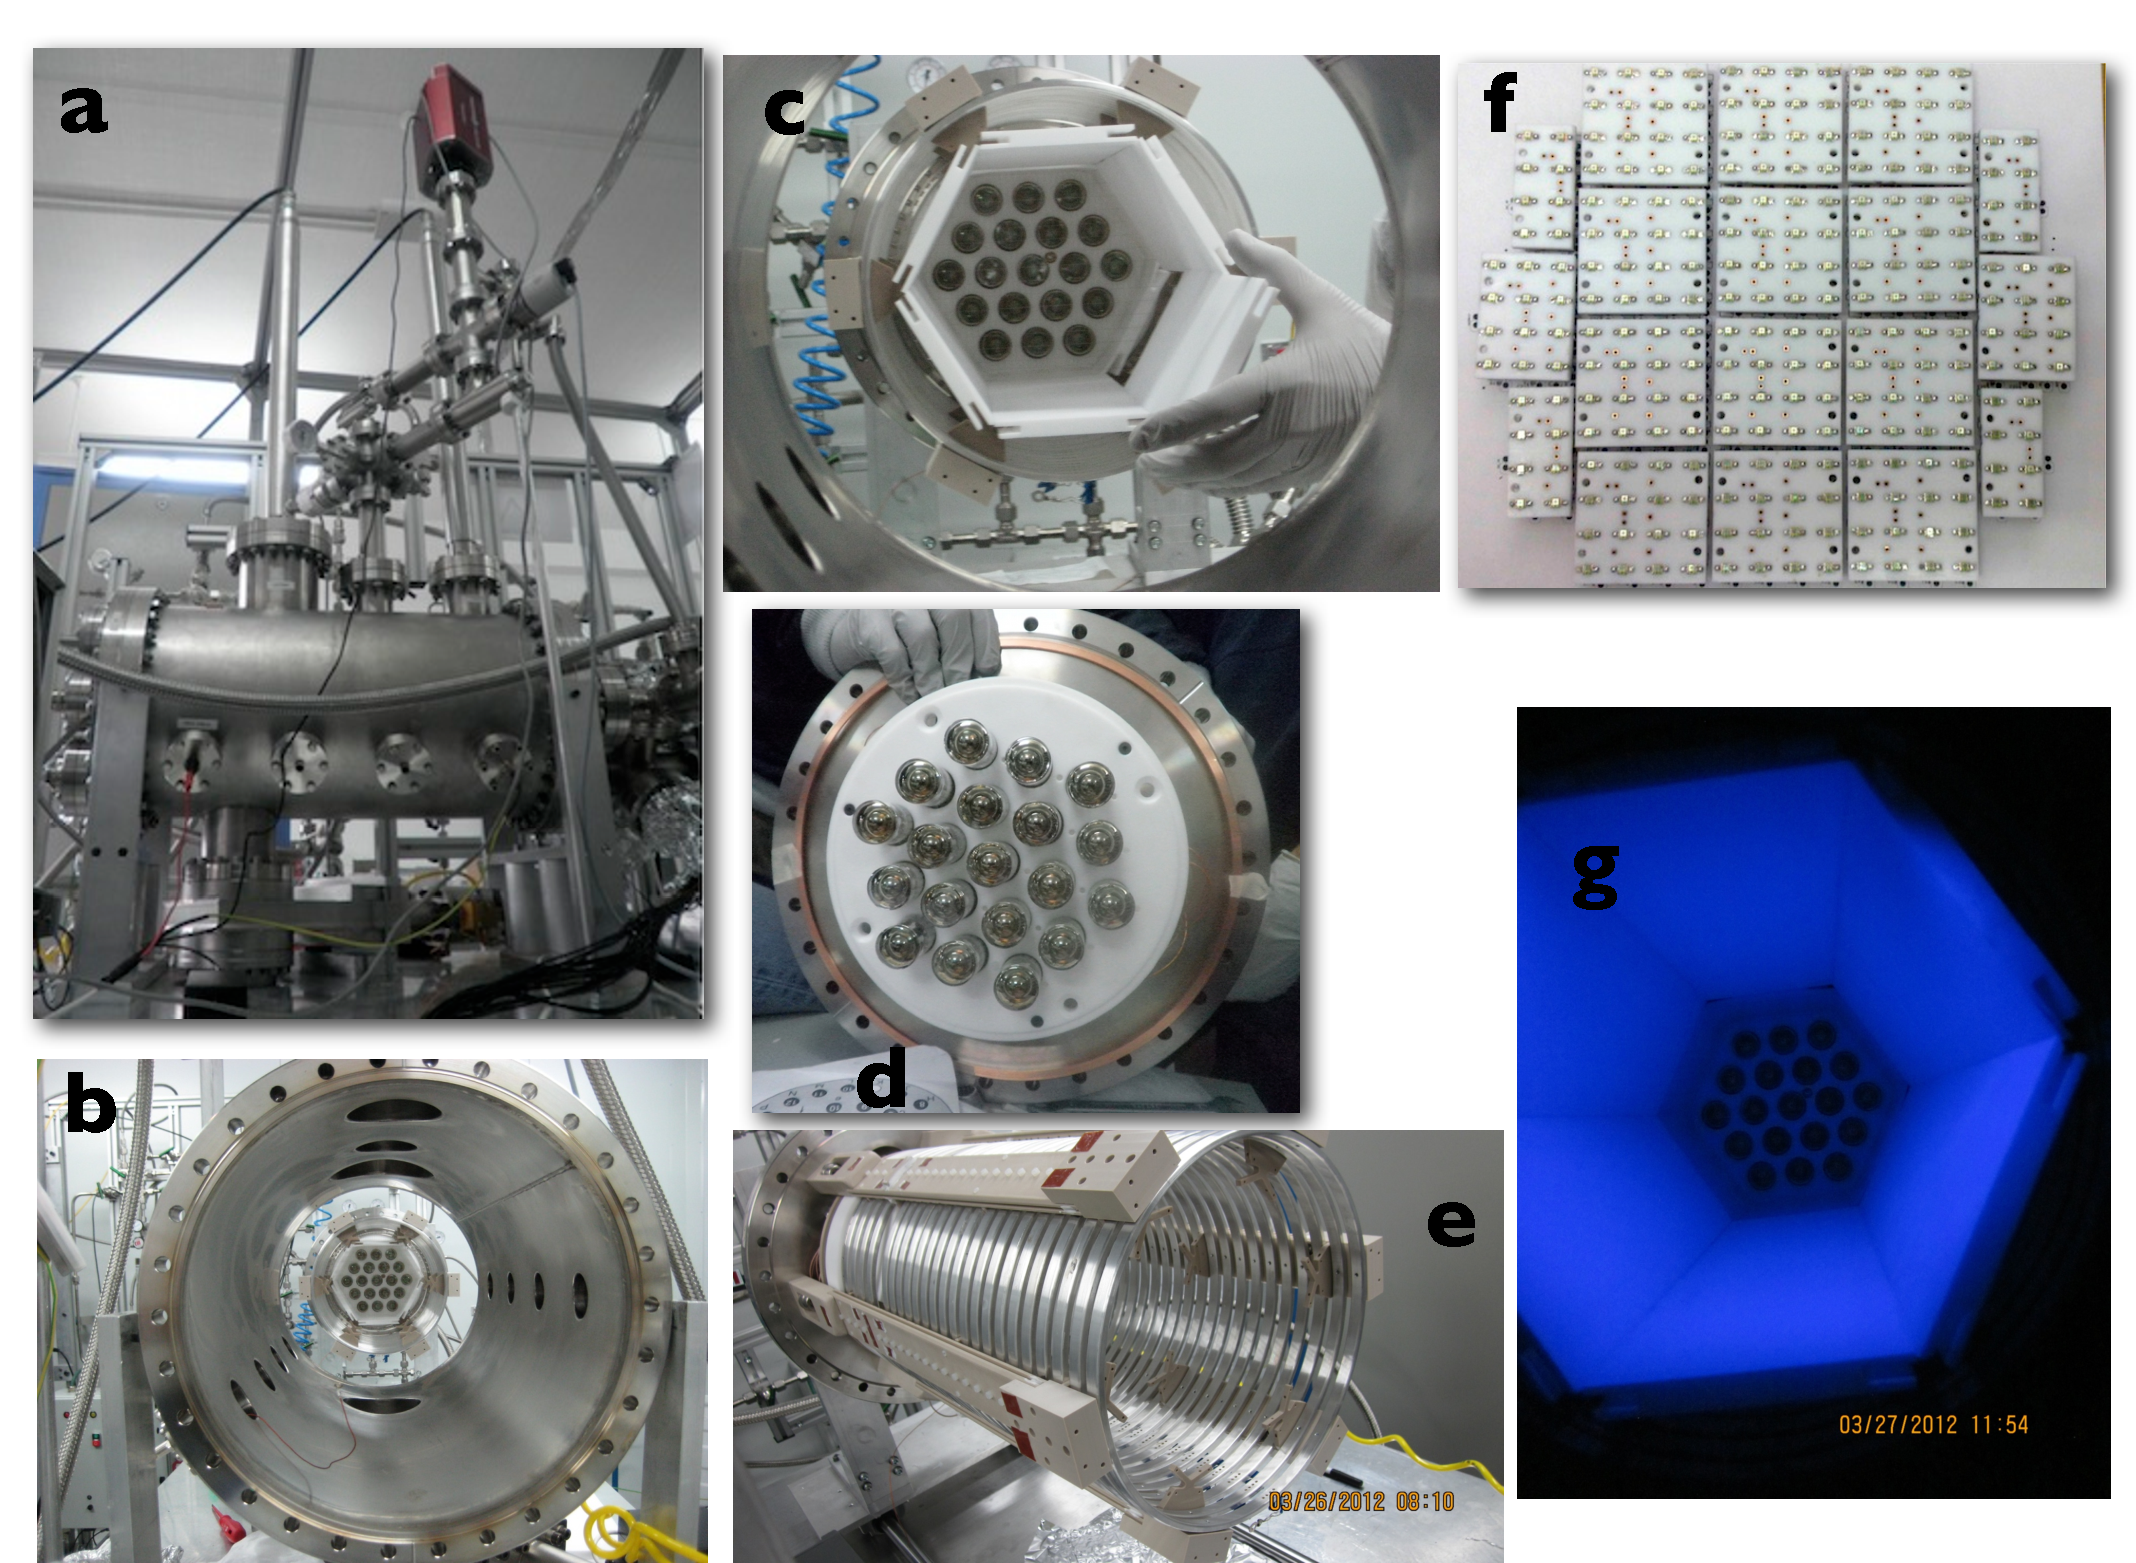
\includegraphics[width=0.7\textwidth]{img/DEMO.pdf}
\caption{\small The NEXT-DEMO prototype. (a) The pressure vessel, showing the HVFT and the mass spectrometer; (b) an expanded view of the detector; (c) Teflon light tube; (d) energy plane, made of pressure resistant Hamamatsu R7378A PMTs; (e) field cage; (f) tracking plane equipped with 300 Hamamatsu MPPCs; (g) Light tube coated with TPB, reflecting UV light in blue.} \label{fig.DEMO}
\end{figure}
%%%%%%%%%%

From 2009 to 2013 the NEXT Collaboration has carried out an intense R\&D program that has culminated in the construction, commissioning and operation of the NEXT-DEMO prototype located at IFIC, and the NEXT-DBDM prototype operating at LBNL. The description of these prototypes and the initial results obtained with them have recently been published\footcite{Alvarez:2012hh, Alvarez:2012nd, Alvarez:2012hu}.

NEXT-DEMO, shown in figure \ref{fig.DEMO}, is as a large-scale prototype and demonstrator of NEXT-100. The pressure vessel has a length of 60 cm and a diameter of 30 cm. The vessel can withstand a pressure of up to 15 bar. The maximum capacity of the detector is 10 kg but in its current configuration (the fiducial volume is an hexagon of 16 cm diameter and 30 cm length) it holds 4 kg at 15 bar. NEXT-DEMO is  equipped with an energy plane made of 19 Hamamatsu R7378A PMTs and a tracking plane made of 300 Hamamatsu MPPCs. 

The detector has been operating successfully for more than one year and has demonstrated: (a) very good operational stability, with no leaks and very few sparks; (b) good energy resolution ; (c) track reconstruction with PMTs and with SiPMs coated with TPB; (d) excellent electron drift lifetime, of the order of 20 ms. In summary, the operation of NEXT-DEMO has been instrumental in the development of the required knowledge to design and build the NEXT detector.

The NEXT-DBDM prototype is a smaller chamber, with only 8 cm drift, but an aspect ratio (ratio diameter to length) similar to the NEXT detector. The device has been used to perform detailed energy resolution studies. NEXT-DBDM achieves a resolution of 1\% FWHM at 660 keV and 15 bar, which extrapolates to 0.5\% at \Qbb.

\subsubsection*{Topological signature}

%%%%%
\begin{figure}
\centering
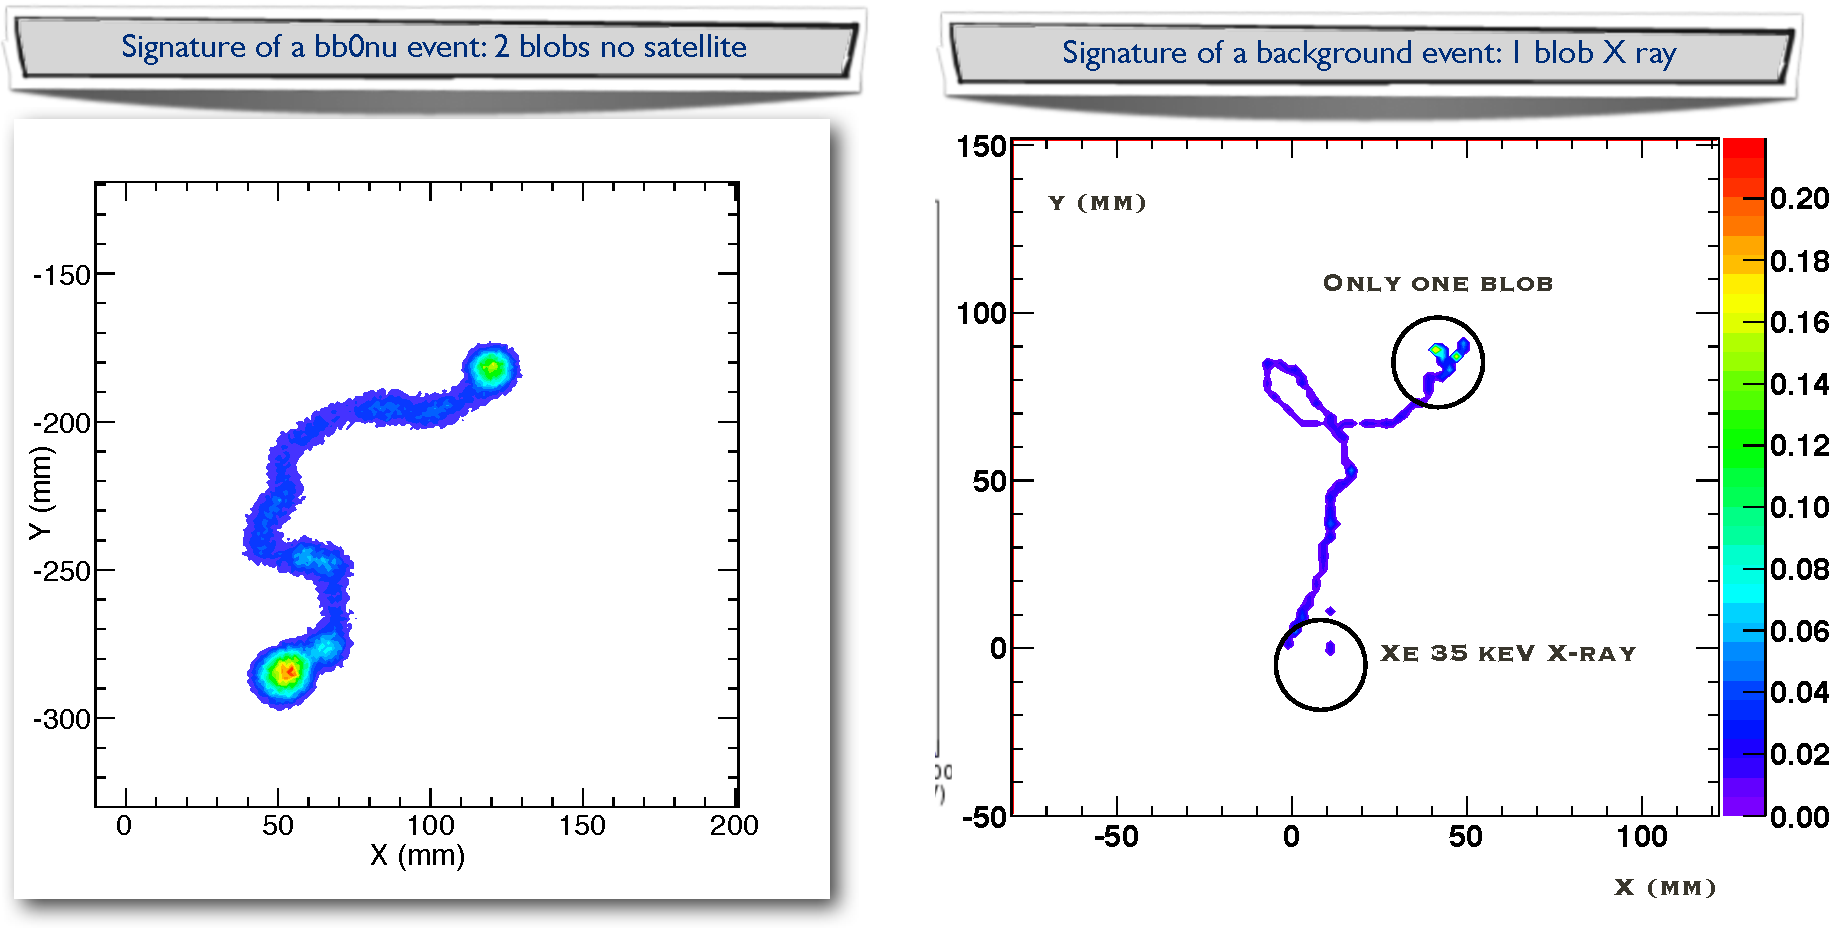
\includegraphics[width=0.9\textwidth]{img/ETRK2.pdf}
\caption{\small NEXT has a topological signature, not available in most \bbonu\ detectors. The panel shows the reconstruction of a Monte Carlo signal (left) and background (right) event. The signal has two electrons (two blobs). The background has only one electron (one blob) and the associated emission of a 35 keV X-ray. The color codes energy deposition in the TPC.}\label{fig.ETRK2}
\end{figure}
%%%%%
	
Double beta decay events leave a distinctive topological signature in HPXe: a continuous track with larger energy depositions (\emph{blobs}) at both ends due to the Bragg-like peaks in the d$E$/d$x$ of the stopping electrons (figure \ref{fig.ETRK2}, left). In contrast, background electrons are produced by Compton or photoelectric interactions, and are characterized by a single blob and, often, by a satellite cluster corresponding to the emission of $\sim30$-keV fluorescence x-rays by xenon (figure \ref{fig.ETRK2}, right).
Reconstruction of this topology using the tracking plane provides a powerful means of background rejection. In our TDR we chose a conservative cut to separate double--blob from single--blob events which provided a suppression factor of 20 for the background while keeping 80\% of the signal.  

The NEXT-DEMO prototype has demonstrated that electron tracks can be easily characterised in an HPXe TPC. Na-22 electrons, with an energy of 511 keV, have been used to demonstrate an efficiency of single-blob counting larger than 98\% and a frequency of erroneous double blob counting of less than 0.14\%. This is a robust confirmation of the excellent background rejection capability of the technology. 

\subsubsection*{Energy resolution}

%%%%%%
%\begin{figure}
%\centering
%\includegraphics[width=0.7\textwidth]{imgs2/RES.pdf}
%\caption{Energy resolution measured with NEXT-DBDM prototype at  15 bar. Data points show the measured energy resolution for 662 keV gammas (squares), 30 keV xenon X-rays (triangles) and LED light pulses (circles) as a function of the number of photons detected. The expected resolution including the intrinsic Fano factor, the statistical fluctuations in the number of detected photons and the PMT charge measurement variance. The measured resolution extrapolates to $\sim$0.5\% FWHM at \Qbb.}\label{fig.RES}
%\end{figure}
%%%%%

%%%%%
\begin{figure}
\centering
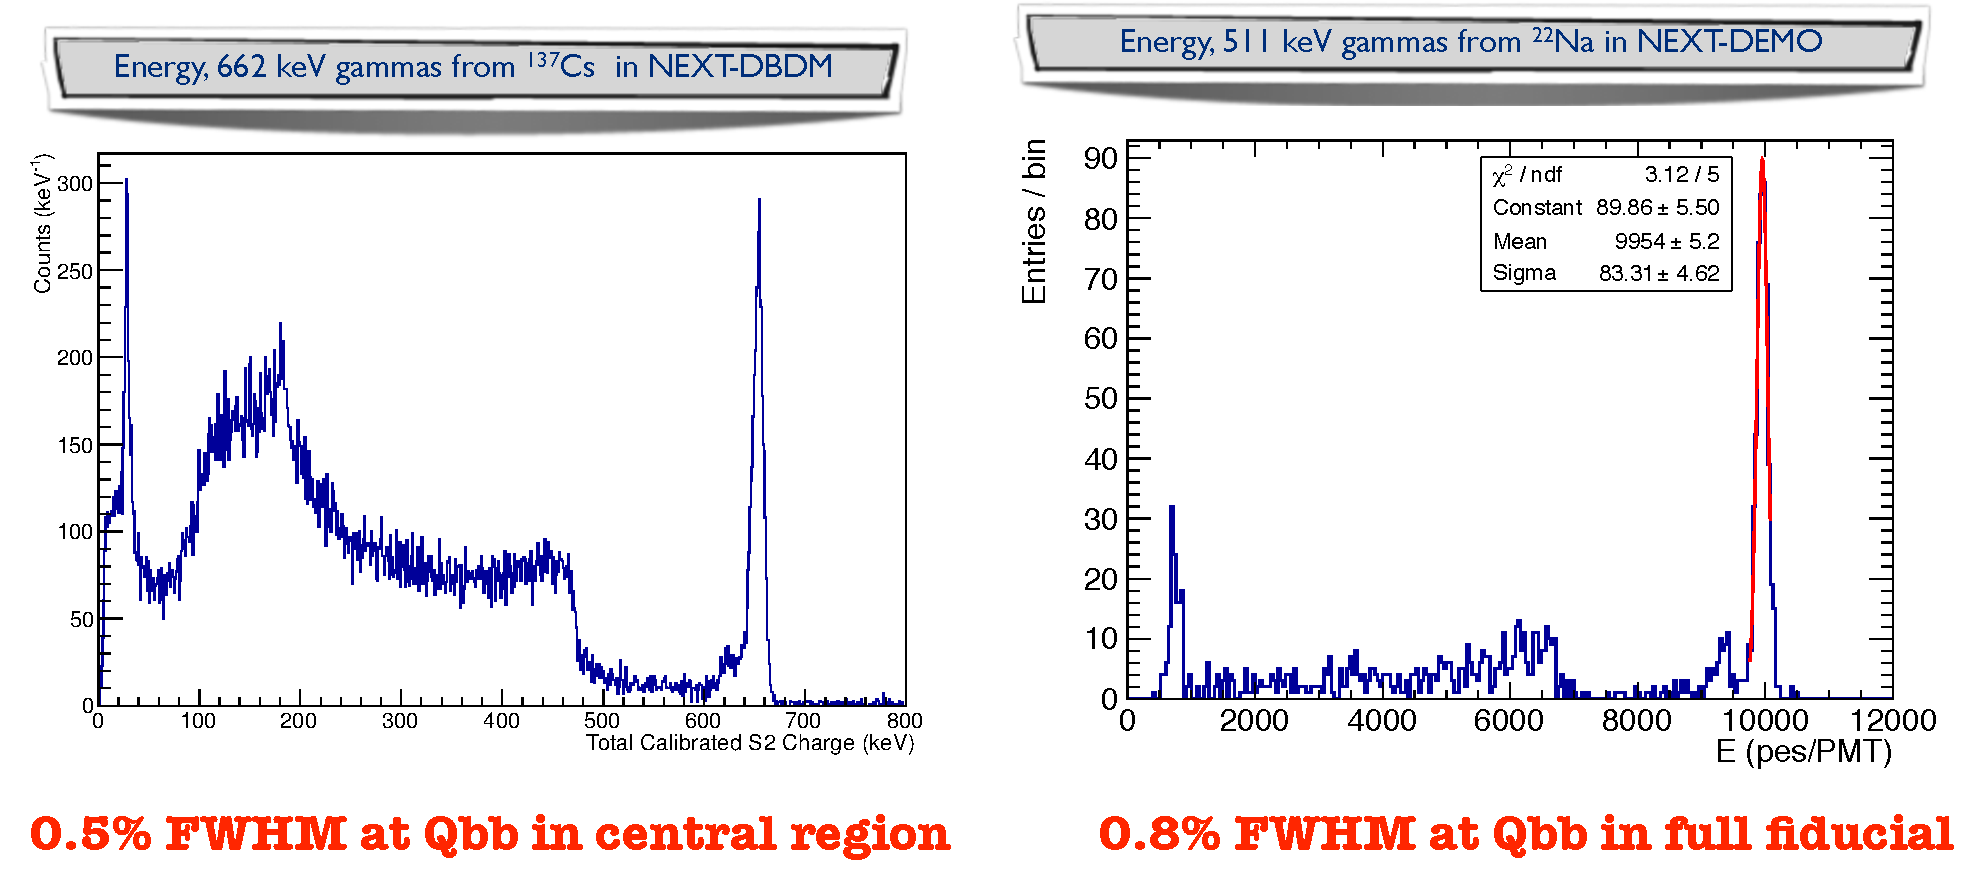
\includegraphics[width=0.9\textwidth]{img/ERS2.pdf}
\caption{\small Left: The resolution of the photo peak for 662 keV electrons in NEXT-DBDM, at 15 bar is 1\% FWHM (0.5\% FWHM at \Qbb); right panel: The resolution of the photo peak for 511 keV electrons in NEXT-DEMO, at 10 bar is 1.9\% FWHM (0.8\% FWHM at \Qbb).}\label{fig.ERES}
\end{figure}
%%%%

The resolution studies with the NEXT prototypes are summarized in Figure \ref{fig.ERES}. NEXT-DBDM apparatus has measured a resolution of 1\% FWHM with 
662 keV photons, which extrapolates to 0.5\% FWHM at \Qbb. This result is not far from the expected limit obtained adding in quadrature the different factors that contribute to the resolution (Fano factor, photoelectron statistics and electronic noise). It clearly shows that a resolution two times better than our initial target can be obtained. NEXT-DEMO measures a resolution of 1.8\% FWHM with 
511 keV photons, which extrapolates to 0.8\% FWHM at \Qbb. The fiducial volume of NEXT-DEMO is much larger than that of NEXT-DBDM and its aspect ratio (the ratio of diameter to length) is only 1/4 of the smaller prototype (whose aspect ratio is, however, close to that of NEXT-100). As a consequence, NEXT-DEMO collects about 3 times less light than NEXT-DBDM, a factor that enters photoelectron statistics and affects geometrical corrections. However, the resolution obtained by the larger prototype is already better than the target of 1\% FWHM described in the TDR.